\chapter{Introduction}
\section{Characteristics of a flow sensor}

There are 2 types of moving media \cite{handbook}:
\begin{itemize}
	\item liquids. \textit{Ex:} water, oil, gasoline.
	\item air and gas. \textit{Ex:} \ce{O2}, \ce{N2}, \ce{CO2}, \ce{CH4}.	
\end{itemize}

Although flow sensors may be simple as detecting velocity of the fluid or air/gas, 
\section{Several examples of flow sensors}
\subsection{Pressure gradient technique}
This technique is applicable only for measuring \textbf{steady flow of nonviscous, incompressible medium} using Bernoulli equation, which relates to \textit{flow resistance}. The working principle of this technique is as follows:
\begin{enumerate}
	\item Create a medium impeding the flow motion in a section of the pipe, such as orifices, porous plugs, and Venturi tubes.
	\item Place 1 differential pressure sensor between the normal sections or 2 absolute pressure sensors in each normal section of the pipe.
	\item Because the high resistance area creates a slight pressure difference in the flow, the mass transferred through the pipe can be estimated.
\end{enumerate}
\begin{figure}[ht]
	\centering
	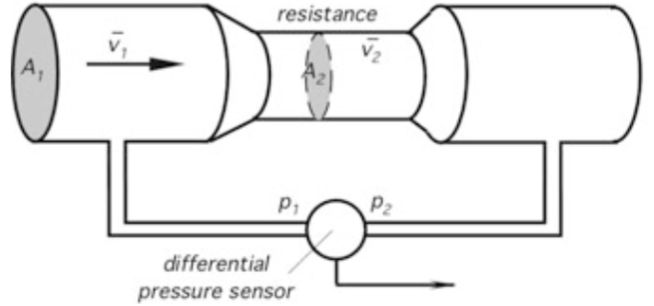
\includegraphics{pressure gradient}
	\caption{Pressure gradient technique example using narrow channel flow \cite{handbook}}
	\label{fig:01}
\end{figure}

The equation for finding mass flow is:
\begin{equation}
q = \epsilon A_2 \sqrt{\Delta p}
\end{equation}

where
\begin{itemize}
	\item $ q $ is the mass flow per unit time,$ \unit{kg/s} $.
	\item $ \epsilon $ is the calibration coefficient.
	\item $ A_2 $ is the cross section of the high resistance area,$ \unit{m^2} $.
	\item $ \Delta p$ is the pressure difference,$\unit{Pa} $.
\end{itemize}

Derivation of the equation is provided in chapter 12 \cite{handbook}.

Advantage of the pressure gradient method is in the absence of moving components and use of standard pressure sensors that are readily available. A disadvantage is in the restriction of flow by a resistive device.

\subsection{Thermal transport sensors}
Thermal transport sensors work by "marking" the flowing medium and detecting the movement of the mark. They are also called \textit{thermoanemometers}. Thermoanemometers are sensitive and have a broad dynamic range. Since the "mark" moves, no moving component is required and low flow rates can also be measured, unlike pressure differential sensors. Another benefit is detection of material change in composition.

A thermoanemometer design determines its operating limit. The upper limit of FSO is determined experimentally.

Data processing system for thermoanemometers must receive at least 3 variable input signals: a flowing medium temperature, a differential, a heating power signal. The signals are multiplexed (i.e. MISO operation), converted into digital form, and processed by a computer to calculate characteristics of flow, displayed in velocities, volume rates or mass rate
\subsubsection{Hot-wire/hot-film Anemometers}
It is a single-part sensor. The wire resistance typically is $ 2-3 \unit{\Omega} $. The operating principle is based on warming up the wire by electric current to $ 200-300\degc $. No media temperature compensation is required. As the flow moves through the wire, it reduces the temperature of the hot wire. The faster the media flows, the stronger the cooling. This phenomena is also known as \textit{forced convection}.

There are 2 methods of controlling temperature and measuring a cooling effect: constant voltage and constant temperature.
\begin{itemize}
	\item Constant voltage: reduction in the wire temperature is measured while the voltage between 2 ends of the wire is constant.
	\item Constant temperature: the temperature remains constant. The power feeds to the wire compensates for temperature loss.
\end{itemize}
The compensating voltage $ \delta V $ for a small change in resistance $ R_w $ is:
\[
\delta V = V_{out}\left(\dfrac{R_w+\delta R_w}{R_w+\delta R_w +R_1} - \dfrac{R_w}{R_w + R_1}\right) \approx V_{out} \dfrac{\delta R_w}{R_w + R_1}
\]
Then, relation between $ R_w $ and temperature change of the hot wire is obtained through experiments and in-depth research regarding the topic.
\begin{figure}[ht]
	\centering
	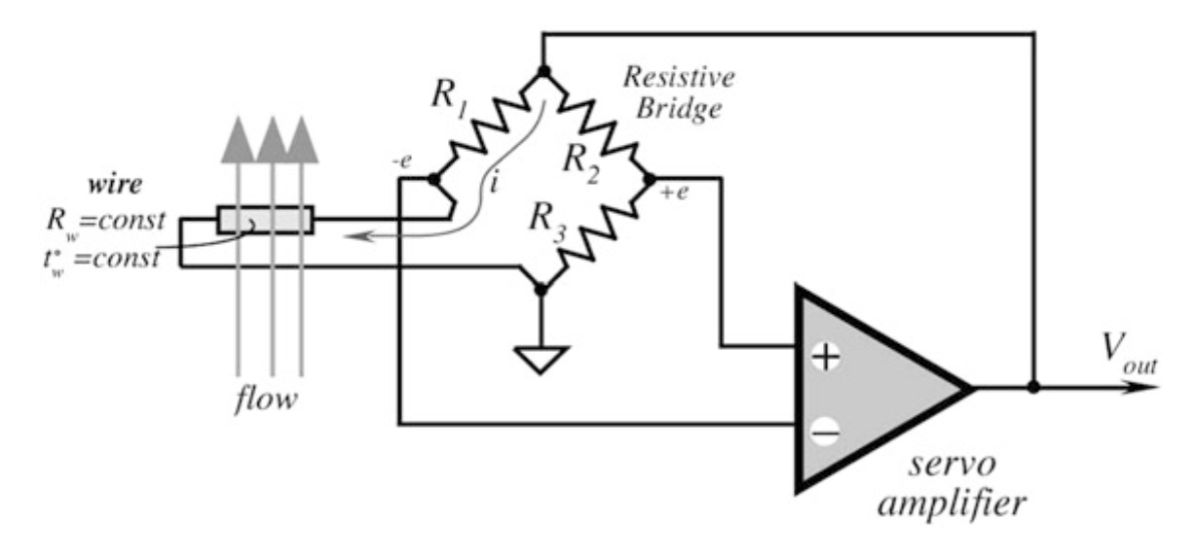
\includegraphics{nullbalanced}
	\caption{Null-balanced bridge for a constant temperature hot-wire anemometer \cite{handbook}}
	\label{nullb}
\end{figure}
Typical design of the hot-wire sensor is shown in \textbf{Figure \ref{hotwire}}. Common materials for the wires are:
\begin{itemize}
	\item tungsten. The wires are strong and have high temperature coefficient ($ 0.004^\circ\text{C}^{-1} $). However, they are prone to high temperatures in many gases due to poor oxidation resistance. This is the most common material at present.
	\item platinum. The wires have high oxidation resistance and temperature coefficient ($ 0.003^\circ\text{C}^{-1} $). However, they are weak, especially at high temperatures.
	\item Platinum-iridium alloy. The wires have good oxidation resistance and are more durable than platinum. However, they have low temperature coefficient ($ 0.00085^\circ\text{C}^{-1} $)
\end{itemize}
\begin{figure}[ht]
	\centering
	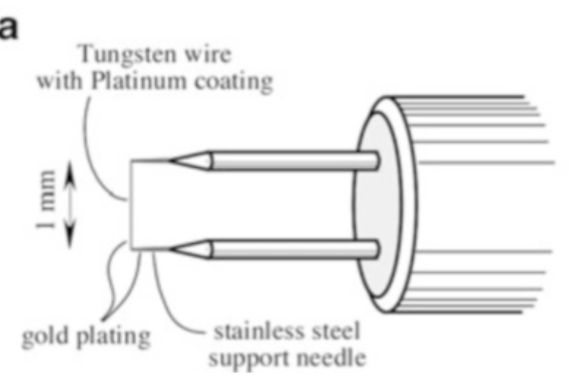
\includegraphics{hotwire 1}
	\caption{Hot-wire probe typical design \cite{handbook}}
	\label{hotwire}
\end{figure}

Typical design of hot-film sensor is shown in \textbf{Figure \ref{hotfilm}}. A common material for the film layer is platinum. The insulator could be made of ceramic substrate.
\begin{figure}[ht]
	\centering
	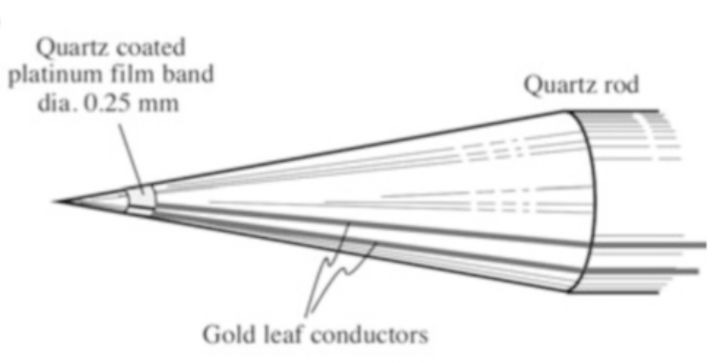
\includegraphics{hotfilm}
	\caption{Hot-film probe with cone-shaped design \cite{handbook}}
	\label{hotfilm}
\end{figure}

The hot-film sensor has several advantages over hot-wire sensor:
\begin{itemize}
	\item Better frequency response due to large surface area with the same rod diameter.
	\item Lower heat conduction to the supports due to low thermal conductivity of the substrate material.
	\item More flexible configurations (e.g. wedge, conical, parabolic shapes).
	\item Less susceptible to fouling and easier to clean.
\end{itemize}

\subsubsection{Three-part Thermoanemometer}
\begin{figure}[ht]
	\centering
	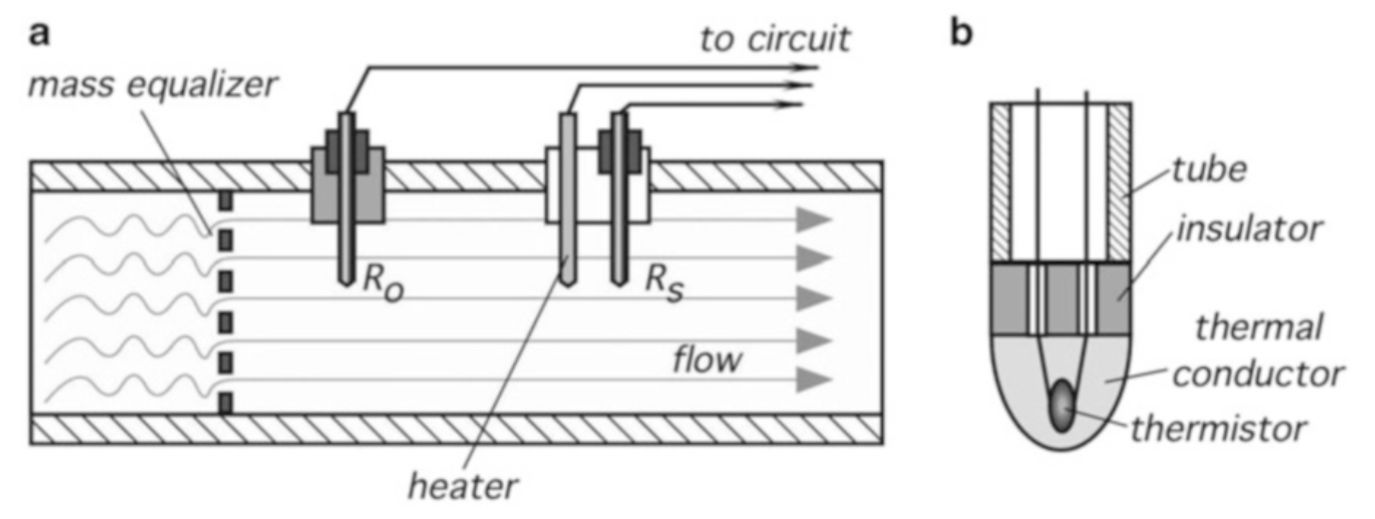
\includegraphics{threepart}
	\caption{Schematic representation and cross-sectional view of a three-part themoanemometer \cite{handbook}}
	\label{3part}
\end{figure}

This type of thermoanemometer is used primarily for liquids but can also be used for gases. The design makes it resistant to contaminated environments. The temperature detector $ R_o $ measures the current temperature of the flowing medium. The heater then warms up the medium and the elevated temperature is measured by the second temperature detector $ R_s $. Through convection phenomena, the amount of heat dissipation is converted to the flow rate of the medium. However, laminar flow must be obtained before measurements for accurate result.

In industry and scientific measurements, resistance temperature detectors (RTDs) is preferable for higher linearity, predictable response and long-term stability over a broader temperature range.

In medicine, thermistors are often preferred for higher sensitivity.

\subsubsection{Two-part Thermoanemometer}

\begin{figure}[ht]
	\centering
	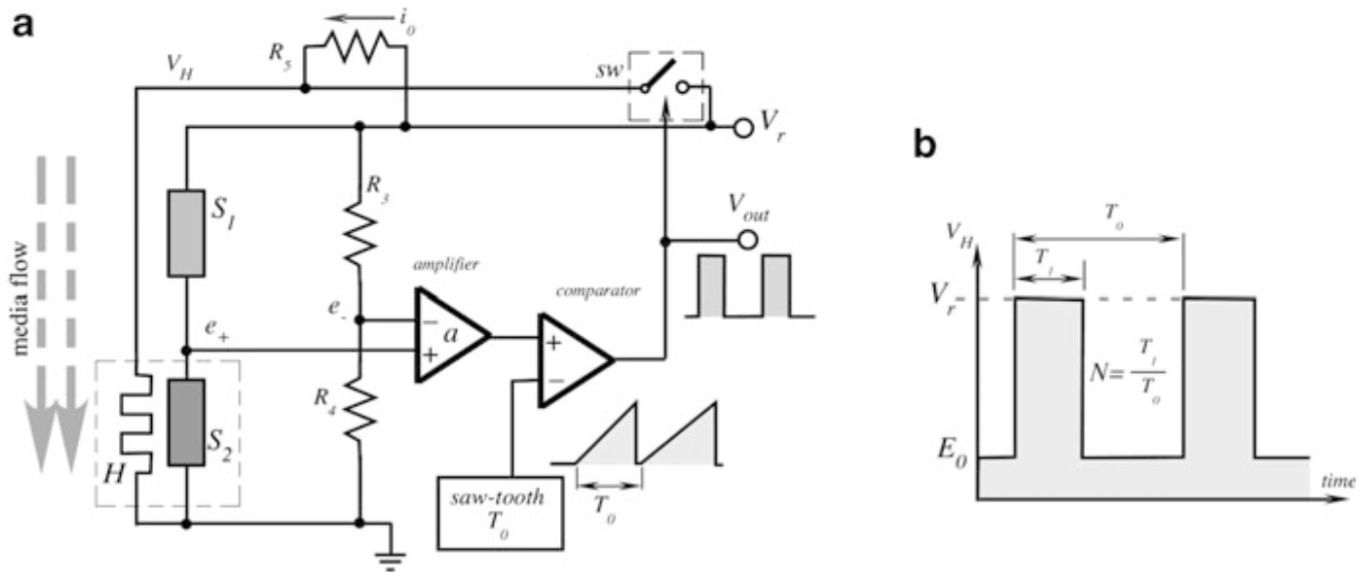
\includegraphics{2part}
	\caption{Control circuit of a themoanemometer with PWM modulator \cite{handbook}}
	\label{2part}
\end{figure}

Fast-response sensors like hot-wire and hot-film sensors are expensive and delicate. More robust and resistant sensors without need of responsiveness (about $ 0.5\unit{s} $) requires different design approaches. The working principle of two-part thermoanemometers is similar to three-part thermoanemometer: measuring temperature of the flowing media; heating the media; monitoring the cooling effect caused by the flow. However, the heat and the second temperature sensor are combined into one sensor.

The thermoanemometer works by a control circuit with a Wheatstone bridge. It generates an output PWM signal where the duty cycle $ N $ represents the airflow rate.

Another thermoanemometer used in precise semiconductor manufacturing is microflow thermal transport sensors. This sensor is developed with MEMS technology. This topic is very advanced and beyond the scope of this report.

\subsection{Ultrasonic Sensors}
The working principle of the sensor can be categorized in 2 ways:
\begin{itemize}
	\item detection of frequency. It uses Doppler effect.
	\item phase shift caused by flowing medium. It relies on the detection of the increase or decrease in effective ultrasound velocity in the medium. 
\end{itemize}
To use the sensor, it is desirable to calibrate the ultrasonic sensors with actual fluids over the useful temperature range so that contribution of a fluid viscosity is accounted for.

\subsection{Electromagnetic Sensors}
\begin{figure}[ht]
	\centering
	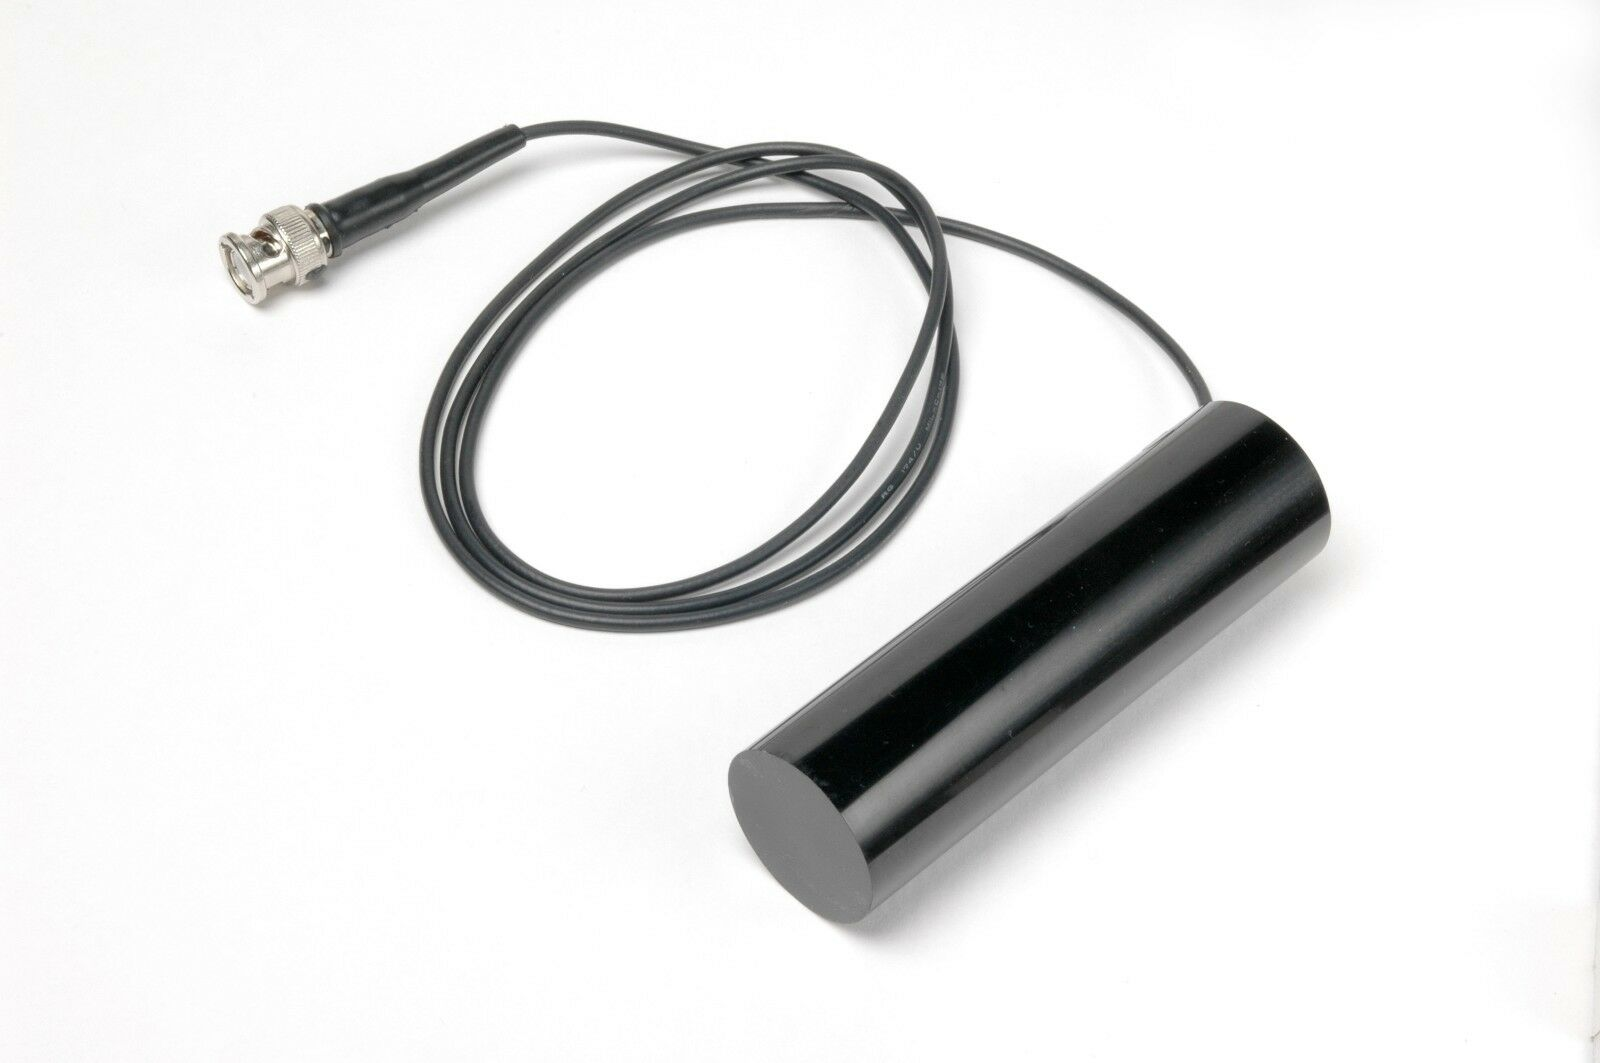
\includegraphics{s-l1600}
	\caption{Electromagnetic sensors MC162}
	\label{electro}
\end{figure}
The electromagnetic flow sensors are useful for measuring the movement of conductive liquids. The operating principle is based on the discovery of Faraday and Henry of the electromagnetic induction. The voltage is induced with an alternating magnetic field. The frequency of magnetic field must be at least 2 times higher than the highest frequency of flow rate variations (Nyquist frequency). This value is typically around $ 100-1000\unit{Hz} $.

\subsection{Breeze Sensors}
\begin{figure}[ht]
\centering
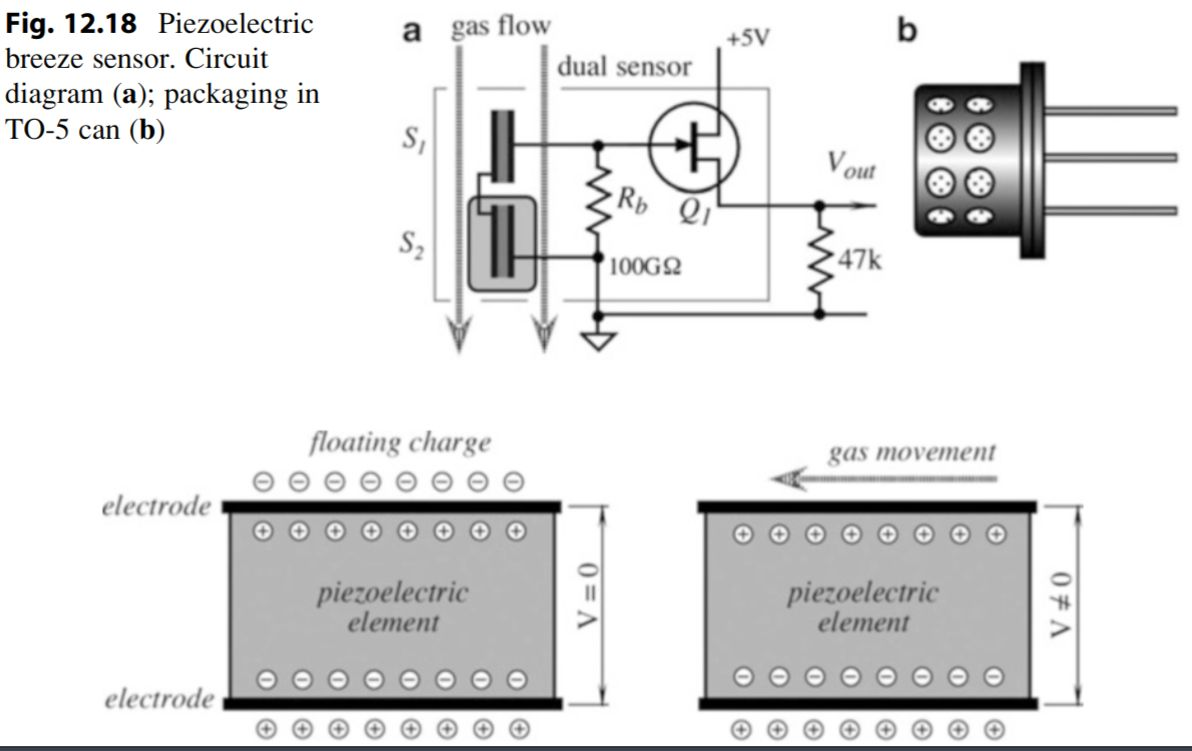
\includegraphics{piezo}
\label{piezo}
\end{figure}
Breeze sensors are used when detection of change in the air/gas movement is needed but not its instantaneous velocity. Gas movement strips off electric charges from surface of piezoelectric element. The voltage induced by piezoelectricity phenomena is applied to the JFET follower creates an output signal at the terminal.

\subsection{Coriolis Mass Flow Sensors}
\begin{figure}[ht]
	\centering
	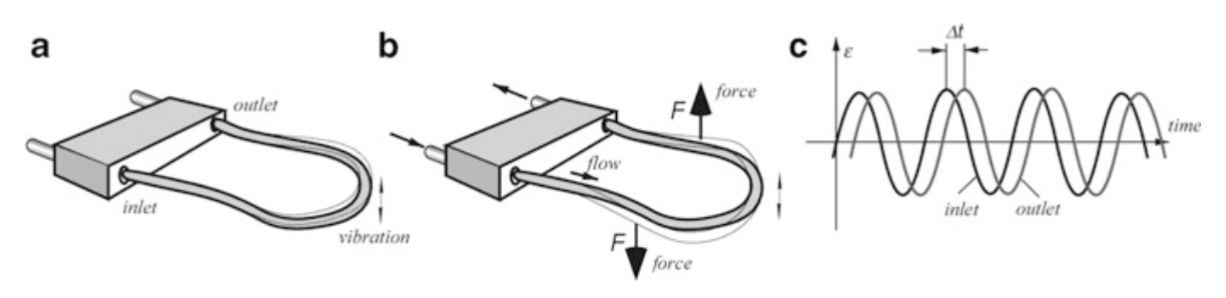
\includegraphics{coriolis}
	\caption{Coriolis sensor's working principle. The phase shift relates to the mass flow}
	\label{coriolis}
\end{figure}
The sensors measure flow of mass directly. Since they are essentially unaffected by the fluid pressure, temperature, viscosity and density, the sensors can be used without recalibration and without compensating for parameters specific to a particular type of fluid. Moreover, gas applications can benefit greatly with these sensors. The Coriolis force is calculated using the following equation:
\[
F = 2m\omega \nu
\]
where $ m $ is the mass, $ \omega $ is the rotation speed, $ \nu $ is the vector of the average fluid velocity. The design of this sensor is shown in \textbf{Figure \ref{coriolis}}. Although having many great advantages, the cost of the sensor is high (about 60,000,000 VND). Therefore, depending on application types (such as measuring multiple fluids), the usage value can offset the initial price.
\begin{figure}[ht]
	\centering
	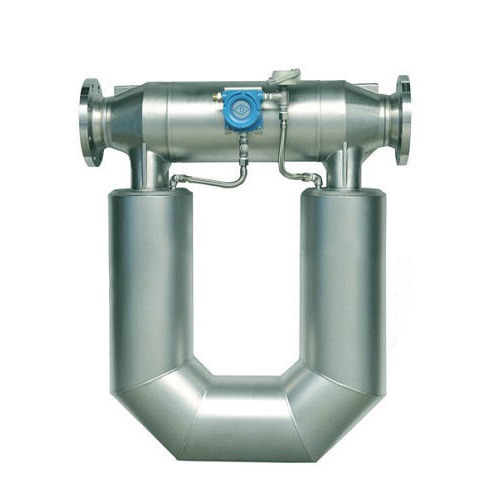
\includegraphics[width=0.5\linewidth]{coriolisfig}
	\caption{Coriolis mass flow sensor}
	\label{coriolisfig}
\end{figure}

\subsection{Drag Force Flowmeter}
\begin{figure}[ht]
	\centering
	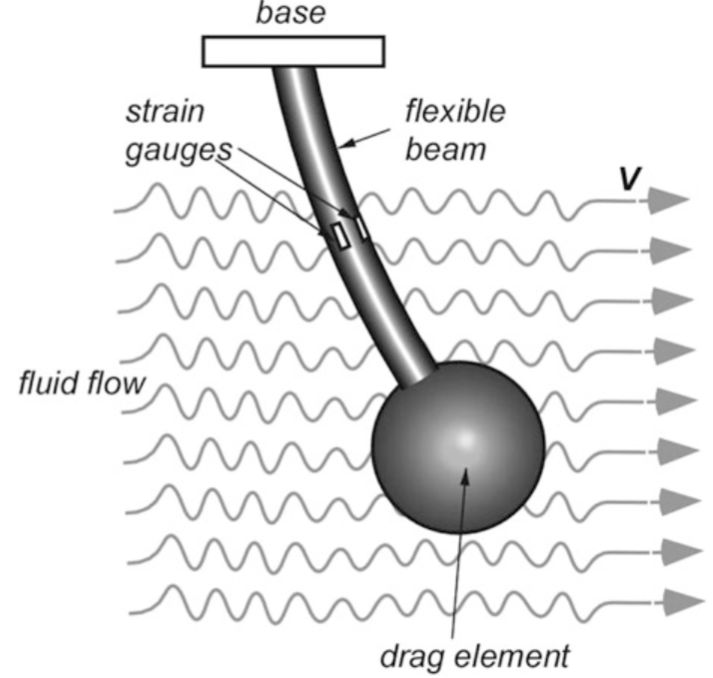
\includegraphics[width=0.5\linewidth]{dragforce}
	\caption{Schematic of the drag force sensor}
	\label{drag}
\end{figure}
For sporadic, multi-directional, turbulent fluids, a drag force flow is efficient. However, it requires environmental monitoring, meteorology, hydrology, maritime studies to measure speeds of air or water flow and turbulence close to surface. The force exerted by the fluid on the drag element is measured (strain measurement of deformation) and converted to an electrical signal indicative of a value for flow speed. This approach can measure 3 dimensional flow instead of 1 dimension like other sensors. A variation of this sensor using MEMS technology is cantilever MEMS sensors, which is again, beyond the scope of the report.

\subsection{Dust and Smoke Detectors}
Although airflow is not monitored, their operation requires movement of gases through the detection chamber of the sensor. To detect presence of small particles suspended in the air, their are 2 types of sensors are widely employed: ionization and optical detectors.
\subsubsection{Ionization Detectors}
\begin{figure}[ht]
	\centering
	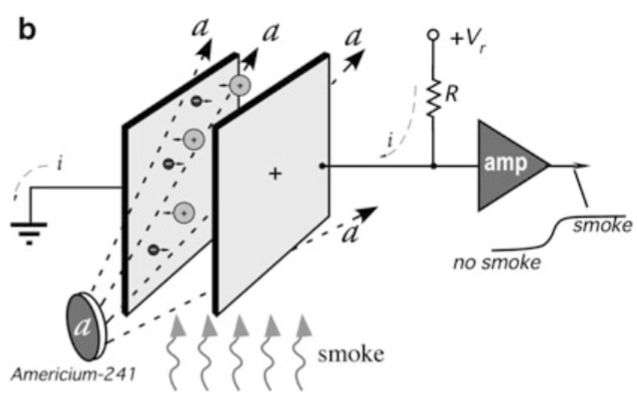
\includegraphics{ionize}
	\caption{Schematic representation of ionization process in smoke detectors}
	\label{ion}
\end{figure}
An ionization chamber containing Americium-241. The radioactive isotope produces alpha particles with a half-life of 432.2 years. If no smoke goes through the space between 2 plates, the alpha particles emanated by Americium-241 ionizes the air molecules by breaking them into positively charged ions and negatively charged electrons. This creates a small current or "virtual wire" for the voltage source $ V_r $ goes to the ground on the left side plate.

If smoke goes through the space between 2 plates, the alpha particles can no longer ionize the air molecules inside the chamber, thus cutting off the "virtual wire". The voltage source then goes through the amplifier "amp", indicating that smoke exists in the room.

\subsubsection{Optical Detectors}
\begin{figure}[ht]
	\centering
	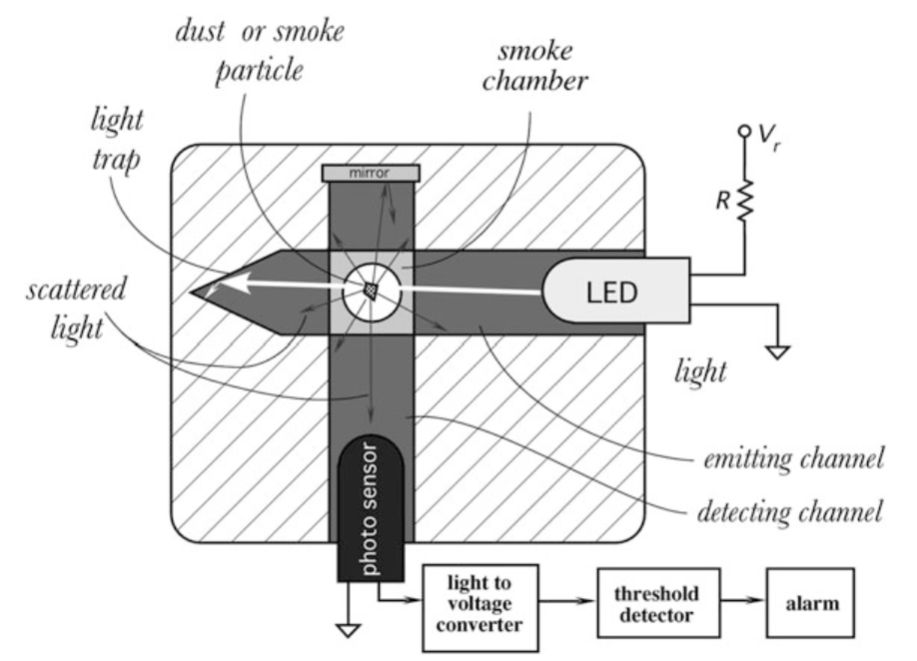
\includegraphics{optic}
	\caption{Cross section of an optical smoke detector. The photosensor and LED could be crossed at less than 90 degree at the expense of mechanical complexity \cite{handbook}}
	\label{optic}
\end{figure}
The effect is the same with optical detectors. If the light source is obstructed from the detector by the smoke, it signals that there is smoke inside the room. However, distinguishing the light coming from the emitter and ambient light with the scattered light from the smoke is the main problem. A possible design is illustrated in \textbf{Figure \ref{optic}}. Depending on the designer's implementation, each smoke detector will have different positioning schemes.

For responding to the light pulses resulted from larger particles, the electronic interface circuit should have a sufficiently wide frequency bandwidth. The optical smoke detectors are less prone to false alarm resulted from steam or cooking fumes in kitchen than the ionization smoke alarms